\documentclass[preprint,12pt,authoryear]{elsarticle}

\linespread{1.25}
\usepackage[text={170mm,220mm},centering]{geometry}
\usepackage{lineno,graphicx}
\usepackage{booktabs}
\usepackage{tabularx}
\usepackage{amssymb,amsmath,amsthm,amsfonts}
\usepackage{subfigure,epsfig}
\usepackage{float}
\usepackage[export]{adjustbox}
\usepackage{url}
\usepackage{setspace}
\usepackage{xspace}
\usepackage{algorithm}
\usepackage{algorithmic}
\usepackage{multirow}
\usepackage{makecell}
\usepackage{xcolor}
\usepackage{svg}
\usepackage[hypertexnames=false]{hyperref}
\hypersetup{hidelinks}

\newtheorem{theorem}{Theorem}
\newtheorem{proposition}{Proposition}
\newtheorem{thm}{Theorem}
\floatplacement{algorithm}{H}
\setlength{\floatsep}{0pt}
\setlength{\textfloatsep}{0pt}
\setlength{\intextsep}{0pt}

\journal{Expert Systems with Applications}

\begin{document}

\begin{frontmatter}

\title{A multi-period vehicle routing problem with dynamic node-road damage for emergency material delivery}

\author{} 
\affiliation{organization={},
            addressline={},
            city={},
            postcode={},
            state={},
            country={}}

\begin{abstract}
Timely emergency material delivery is difficult when affected demand nodes and transportation links both evolve over time. A route that is short in distance may still generate large rescue losses if high-urgency nodes are served late or if vehicles traverse severely damaged roads. This paper studies a multi-period vehicle routing problem with dynamic node-road damage, where rescue vehicles and relief inventories are released in repeated dispatch periods rather than being fully available at the beginning of the horizon. This period structure is operationally important because single-period aggregation can overestimate early rescue capacity and underestimate dynamic loss. Node damage is modeled as an arrival-time-dependent recovery-deterioration process, and road damage affects vehicle speed and downstream arrival times. To solve the problem, we develop an improved hybrid genetic algorithm (IHGA) that embeds damage-critical, period-aware, and route-structure-aware repair moves into a population-based HGA framework. Experiments on Solomon-type C, R, and RC instances show that IHGA consistently obtains lower dynamic damage than Omega-VNS and ESWA-IMA. On C101-25, r101-25, and rc101-25, IHGA reduces average dynamic damage by 1.31\%, 2.22\%, and 2.30\% relative to IMA, and by 7.07\%, 8.32\%, and 6.78\% relative to VNS. Ablation results further show that the proposed repair operators improve average damage on C, R, and RC layouts. Model-comparison experiments further show that the damage-oriented model reduces dynamic damage by 13.10\%--20.28\% relative to a cumulative-arrival-time-oriented CCVRP baseline and by 19.33\%--26.63\% relative to a distance-oriented CVRP baseline. Multi-period sensitivity experiments further show that an aggregated single-period model gives an optimistic lower-bound estimate because it assumes all vehicles and supplies are available at time zero. Under staged dispatch, the same total resources cause higher dynamic damage as vehicles and inventories are released in later waves. These results demonstrate the value of explicitly modeling dynamic damage and staged multi-period dispatch in emergency routing decisions.
\end{abstract}

\begin{highlights}
\item A multi-period emergency routing model captures staged vehicle dispatch and period inventory release.
\item IHGA uses urgency-aware construction with damage-critical, period-aware, and route-structure repair.
\item Damage-oriented routing outperforms VNS, IMA, CVRP, and CCVRP baselines on C, R, and RC instances.
\item Ablation isolates the contribution of damage-critical and period-aware repair operators.
\item Sensitivity results quantify optimistic aggregation bias, period splitting, vehicle supply, and inventory thresholds.
\end{highlights}

\begin{keyword}
Multi-period vehicle routing \sep emergency logistics \sep dynamic damage \sep hybrid genetic algorithm \sep sensitivity analysis \sep Solomon instances
\end{keyword}

\end{frontmatter}

\section{Introduction}
\label{sec:introduction}

Emergency material distribution differs from ordinary vehicle routing because delay has a direct loss consequence. After a disaster, affected locations continuously change their states: a demand point may deteriorate if it is not served, while the arrival of supplies may reduce the expected loss. Transportation links also change over time. A damaged road can reduce travel speed and delay all nodes scheduled after that link. Therefore, minimizing geographical distance alone is insufficient for disaster-response routing. The routing policy must decide not only which vehicle serves which demand node, but also in which period the node is served, which link alternative is selected, and how limited supplies are allocated over time.

The multi-period structure is not a secondary parameter in this setting. In realistic emergency response, all vehicles and supplies are rarely available at time zero. Rescue capacity is released in waves because vehicles return, roads are cleared gradually, and inventories arrive through staged procurement or upstream transport. If the planning horizon is collapsed into a single period, the model implicitly allows later-period vehicles and supplies to be used immediately, creating an optimistic dispatch plan and hiding the loss caused by delayed resource availability. A multi-period model is therefore needed to represent when resources can actually be used, not only how many resources exist in total.

This study considers a multi-period vehicle routing problem with dynamic damage. The problem is motivated by emergency material delivery where a dispatch center repeatedly sends rescue vehicles to affected nodes. Each node has demand, service time, initial damage, deterioration rate, and recovery rate. Each pair of nodes is connected by multiple road alternatives, and each road alternative has an initial damage and deterioration trajectory. The resulting decision problem couples vehicle routing, period assignment, road selection, period inventory allocation, and dynamic loss evaluation.

The main challenge is that the objective is not a static sum of arc distances. The cost of serving a node depends on its arrival time, and the arrival time itself depends on previous node choices, service times, and road damage. This feedback creates a highly nonlinear combinatorial problem. Moreover, sensitivity analysis is important for emergency planning: decision makers often need to know how much benefit is obtained by adding vehicles, increasing the number of periods, or changing available inventory. A good algorithm should therefore deliver not only low objective values but also stable and interpretable marginal-effect curves.

The contributions of this paper are summarized as follows.
\begin{itemize}
\item We formulate a multi-period routing model in which staged vehicle dispatch, period inventory, dynamic node damage, and dynamic road damage jointly determine rescue loss.
    \item We design an improved hybrid genetic algorithm (IHGA) with urgency-aware initialization, damage-critical relocation/exchange, period relocation, and route-structure repair operators.
\item We introduce damage-critical relocation and exchange operators together with period-aware relocation, diversity refresh, and warm-start transfer, so that high-loss nodes can be moved to earlier feasible periods and resource-sensitivity curves remain stable.
    \item We conduct algorithm comparison, model comparison, sensitivity analysis, and node-priority analysis on C, R, and RC benchmark instances to validate both solution quality and decision-support interpretation.
\end{itemize}

\section{Literature review}
\label{sec:literature}

The vehicle routing problem (VRP) and its variants have been extensively studied since the early development of vehicle routing with time windows \citep{solomon1987algorithms}. Classical VRP models usually optimize distance, travel time, or fleet size under vehicle-capacity and service constraints. Surveys and benchmark studies show that high-quality solutions typically require hybrid metaheuristics that combine population-based search with local improvement procedures \citep{braysy2005vehicle, pisinger2007general, vidal2013hybrid}.

Emergency logistics introduces additional modeling requirements. Relief distribution after disasters is commonly dynamic and time dependent because demand, vehicle availability, and network accessibility change during the response process \citep{ozdamar2004emergency, sheu2007emergency}. Literature reviews also show that post-disaster logistics models frequently combine routing, allocation, inventory, and transportation decisions rather than treating delivery as a static distance-minimization problem \citep{caunhye2012optimization, afshar2012modeling}.

A second important stream concerns the objective function of humanitarian logistics. Since delayed delivery can translate into human suffering, response-time proxies, unmet-demand penalties, deprivation costs, and social-cost objectives have been proposed to better represent disaster-response performance \citep{holguinveras2013objective}. In such settings, the timing of service is central: serving the same node earlier or later may cause very different losses.

This paper is positioned at the intersection of multi-period routing and time-dependent damage evaluation. Compared with distance-minimizing VRP models, the proposed problem evaluates the dynamic state of demand nodes and road links. Compared with standard time-window routing, the loss is a continuous function of arrival time instead of a hard feasibility interval. Compared with single-period emergency routing, the model explicitly represents repeated dispatch periods and period-level inventory constraints, which prevents later resources from being treated as if they were available in the first dispatch wave.

\section{Problem description and modeling}
\label{sec:model}

Let $G=(N_0,A)$ be a complete directed graph, where $N=\{1,\ldots,n\}$ is the set of affected demand nodes and node $0$ denotes the depot. The planning horizon is divided into $P$ dispatch periods. Period $p$ starts at $T_p=(p-1)\Delta$, where $\Delta$ is the period-length parameter. In the reported experiments, $\Delta=1440/P$, corresponding to a normalized one-day planning horizon measured in minutes. In each period $p\in\{1,\ldots,P\}$, at most $K$ rescue vehicles can be used. Each vehicle has capacity $Q$, and the available period inventory is $B_p$. In the implementation used in the experiments, $B_p$ is set adaptively according to total demand and the number of periods.

The solution determines the assignment of every demand node to exactly one vehicle route, the service sequence within each route, the dispatch period of each route, and the road alternative selected for each traversed arc. Demand splitting is not allowed: once a node is assigned to a route, the vehicle delivers the full demand of that node.

Each demand node $i\in N$ has demand $q_i$, service time $s_i$, initial damage $a_i$, deterioration rate $b_i$, and recovery rate $\rho_i$. If node $i$ is served at arrival time $A_i$, its remaining damage is evaluated as
\begin{equation}
D_i(A_i)=a_i e^{-\rho_i A_i}+\frac{b_i}{\rho_i}\left(1-e^{-\rho_i A_i}\right).
\label{eq:node-damage}
\end{equation}
This expression captures two competing effects: existing damage is gradually recovered, while unserved demand continues to deteriorate until service.

For each arc $(i,j)\in A$, several road alternatives $z\in Z$ are available. Road alternative $z$ has initial damage $a_{ijz}^{r}$, deterioration rate $b_{ijz}^{r}$, and recovery rate $\rho_{ij}^{r}$. If a vehicle enters the road at time $t$, the road damage is
\begin{equation}
R_{ijz}(t)=a_{ijz}^{r}e^{-\rho_{ij}^{r}t}+\frac{b_{ijz}^{r}}{\rho_{ij}^{r}}\left(1-e^{-\rho_{ij}^{r}t}\right).
\label{eq:road-damage}
\end{equation}
The road state affects the effective speed:
\begin{equation}
v_{ijz}(t)=\left(1-\frac{R_{ijz}(t)\rho_{\min}^{r}}{0.814\,b_{\max}^{r}}\right)v_0,
\label{eq:speed}
\end{equation}
where $v_0$ is the nominal vehicle speed, $\rho_{\min}^{r}$ is the minimum road recovery rate, and $b_{\max}^{r}$ is the maximum road deterioration rate.

Consider a route $r=(0,i_1,i_2,\ldots,i_m)$ dispatched in period $p$. Let $T_p$ be the start time offset of period $p$. The arrival time is recursively computed by
\begin{equation}
A_{i_1}=T_p+\frac{d_{0i_1z}}{v_{0i_1z}(T_p)},
\end{equation}
\begin{equation}
A_{i_{h+1}}=A_{i_h}+s_{i_h}+\frac{d_{i_hi_{h+1}z}}{v_{i_hi_{h+1}z}(A_{i_h}+s_{i_h})},\quad h=1,\ldots,m-1.
\end{equation}

The primary objective is to minimize total weighted node damage:
\begin{equation}
\min F=\sum_{i\in N}\omega_i D_i(A_i)+M\cdot \Phi,
\label{eq:objective}
\end{equation}
where $\omega_i$ is the loss weight of node $i$, $M$ is a large penalty coefficient, and $\Phi$ is the total violation of vehicle-capacity and cumulative period-inventory constraints. The reported experiments use $M=10000$. Road damage is not ignored: it changes speed through Eq.~\eqref{eq:speed}, thereby affecting arrival times and downstream node losses.

The main constraints are as follows:
\begin{align}
&\sum_{r}\sum_{h:i_h=i}1=1, && \forall i\in N, \\
&\sum_{i\in r}q_i\le Q, && \forall r, \\
&\sum_{\tau=1}^{p}\sum_{r\in \mathcal{R}_{\tau}}\sum_{i\in r}q_i\le \sum_{\tau=1}^{p}B_{\tau}, && p=1,\ldots,P, \\
&|\mathcal{R}_{p}|\le K, && p=1,\ldots,P.
\end{align}
The cumulative inventory constraint allows early periods to use only the supplies that have become available by that time. This is the key distinction between the proposed multi-period formulation and an aggregated single-period formulation: the latter only checks whether total supply is sufficient over the whole horizon, whereas the former also checks whether enough supply is available before each dispatch wave. As a result, the model can quantify the loss caused by delayed resource release.

\section{Improved hybrid genetic algorithm}
\label{sec:algorithm}

The proposed IHGA uses a route-based encoding. An individual contains the complete set of routes over all periods. Route index $1$ to $K$ belongs to period 1, route index $K+1$ to $2K$ belongs to period 2, and so on. This fixed route-period mapping is important because route collapse or route renumbering would destroy the multi-period semantics.

\subsection{Initialization}

The initial candidate solutions are generated by combining randomized construction, urgency-aware construction, and distance-structured construction. The urgency score of node $i$ is
\begin{equation}
u_i=a_i+\frac{b_i}{\max(\rho_i,\epsilon)},
\end{equation}
where $\epsilon$ avoids division by zero. Candidate populations combine randomized sequences, weighted urgency sequences, and urgency-ranked sequences with band-level shuffling. During insertion, candidate vehicles are screened by vehicle capacity and cumulative period-inventory feasibility. The insertion cost combines travel distance, current route load, and current route length.

\subsection{Crossover and local search}

The crossover operator identifies two similar routes from two parent solutions and preserves their common nodes. Nodes not preserved are reinserted into feasible routes. This route-similarity crossover is designed to inherit useful route blocks without breaking feasibility.

Local search is applied after crossover. The neighborhoods include intra-route swap, insertion, 2-opt reversal, inter-route exchange, and inter-route relocation. These operators are guided by initial damage and deterioration-rate scores, but random choices are retained to avoid premature convergence. Road selection is improved by both random and greedy road-alternative selection.

\subsection{Damage-critical, period-aware, and high-fleet operators}

Because the problem is multi-period and damage-driven, generic route moves are not enough. IHGA therefore uses operators that directly target late high-loss nodes, period assignment, and excessive route fragmentation.

\textbf{Damage-critical relocation} selects customers with large realized damage, late arrival time, and high urgency score, then tries to move them to earlier feasible positions. Candidate target routes are ranked by period, load, and route length. This operator directly reduces the main objective because it searches around the nodes that currently contribute most to total loss.

\textbf{Damage-critical exchange} swaps a high-loss late customer with a lower-loss earlier customer when the exchange is capacity-feasible and improves the dynamic-damage objective. This operator is useful when direct relocation is blocked by vehicle capacity or period-inventory constraints.

\textbf{Period relocation} moves urgent nodes from later periods to earlier feasible routes. Since each route index is tied to a period, the operator preserves the route-period mapping and evaluates only affected routes after each candidate move.

\textbf{Parallel relocation} is activated when the vehicle number is sufficiently large. It moves urgent nodes from long routes to empty or short routes in the same period, exploiting additional vehicles to reduce arrival times.

\textbf{Route merge and route rebuild} control excessive fragmentation. Route merge combines short same-period routes when vehicle capacity permits, while route rebuild reorders route nodes using urgency-first and nearest-neighbor candidate sequences. These two operators are especially useful on clustered instances where too much parallel splitting may increase downstream travel delay.
\subsection{Warm-start transfer for sensitivity analysis}

Vehicle-number sensitivity analysis should reflect a basic monotonicity property: when more vehicles are available, the feasible solution space expands. Running every vehicle-number level from a completely random population may hide this property and produce artificial fluctuations. To address this, the experiment runner transfers the best solution from a smaller fleet to the first individual of the next larger fleet. Routes are copied period by period while preserving route indices. The larger fleet can then refine the inherited solution by using additional vehicles. This warm-start mechanism stabilizes marginal-effect curves without preventing further improvement.

\begin{algorithm}[H]
\caption{Improved hybrid genetic algorithm}
\label{alg:ihga}
\begin{algorithmic}[1]
\STATE Load instance data, node damage parameters, and road damage parameters.
\STATE Generate an initial population using randomized and urgency-aware construction.
\IF{a warm-start solution is available}
    \STATE Embed the previous best route set into the first individual.
\ENDIF
\STATE Evaluate all individuals using dynamic arrival-time and damage equations.
\FOR{$t=1$ to $T_{\max}$}
    \FOR{each individual in the population}
        \STATE Select a good parent and apply route-similarity crossover.
        \STATE Apply swap, insertion, 2-opt, exchange, and relocation neighborhoods.
        \STATE Apply damage-critical relocation/exchange, period relocation, parallel relocation, route merge, and route rebuild when eligible.
        \STATE Improve road alternatives by random and greedy selection.
    \ENDFOR
    \STATE Update the population and elite best solution.
\ENDFOR
\STATE Polish the global best by period-aware and route-level operators.
\RETURN Best route set and dynamic-damage objective value.
\end{algorithmic}
\end{algorithm}

\section{Experiments}
\label{sec:experiments}

\subsection{Experimental design}
\label{subsec:experimental-design}

The experiments are designed to evaluate both optimization quality and decision-support interpretability. Five groups of experiments are reported, as summarized in Table~\ref{tab:experiment-plan}. The first group compares IHGA with Omega-VNS and ESWA-IMA under the same dynamic-damage objective. The second group isolates the contribution of the proposed repair components through ablation. The third group compares the proposed damage-oriented model with distance-oriented CVRP and cumulative-arrival-time-oriented CCVRP baselines. The fourth group is centered on multi-period resource planning: it analyzes how vehicle number, dispatch-period splitting, and period inventory change dynamic damage. The fifth group examines whether high-urgency nodes are actually served earlier.

\begin{table}[H]
\centering
\caption{Experimental plan.}
\label{tab:experiment-plan}
\small
\begin{tabularx}{\textwidth}{>{\raggedright\arraybackslash}p{0.08\textwidth}>{\raggedright\arraybackslash}p{0.25\textwidth}>{\raggedright\arraybackslash}X>{\raggedright\arraybackslash}p{0.20\textwidth}}
\toprule
No. & Experiment & Purpose & Output metrics \\
\midrule
E1 & Algorithm comparison & Compare IHGA with Omega-VNS and ESWA-IMA under the same data, constraints, and dynamic objective. & Best, average, standard deviation \\
E2 & Operator ablation & Remove the main repair components from MP-IHGA to isolate their contributions. & Average damage, best damage, loss increase \\
E3 & Model comparison & Compare the proposed DDVRP-IHGA model with multi-period CVRP and CCVRP baselines. & Dynamic damage, relative improvement \\
E4 & Multi-period resource sensitivity & Analyze vehicle number, optimistic single-period aggregation, staged dispatch periods, and period inventory on C, R, and RC instances. & Objective, marginal benefit, aggregation bias, period-splitting effect \\
E5 & Node-priority analysis & Divide nodes into urgency groups and test whether high-urgency nodes are served earlier. & Arrival time, node damage, service rank \\
\bottomrule
\end{tabularx}
\end{table}

Unless otherwise stated, the experiments use three Solomon-type benchmark data sets with 100 demand nodes and one depot: C101-25 (clustered), r101-25 (random), and rc101-25 (mixed random-clustered). The default number of planning periods is $P=3$, vehicle capacity is 200, and the base period inventory is $Q_p=\lceil\sum_i q_i/P\rceil$, giving 604, 486, and 575 units for C101-25, r101-25, and rc101-25, respectively. Reported averages use paired independent seeds within each experiment group. The analysis focuses on solution quality and planning interpretation rather than computing-time comparison.

Following the benchmark organization used in the original DCCVRPMRS study \citep{zhao2026routing}, instance expansion is applied to the comparison experiments rather than to every sensitivity experiment. The original study expands the algorithm-comparison, objective-comparison, and heuristic-priority tables across multiple benchmark instances and scales, while using representative scenario experiments for the cluster and sensitivity analyses. A data check showed that same-family Solomon labels such as C101, C102, and C103 are not independent after conversion to the present DDVRP input format because the implementation uses coordinates, demand, service time, and road matrices, but not the original ready-time and due-time-window fields. Therefore, these labels are not used as independent extended evidence. For E1, E2, and the priority-strategy comparison, we instead import three spatially distinct 200-customer Gehring--Homberger benchmark instances from the SINTEF TOP VRPTW archive and truncate each to the first 100 customers, producing HC1-100, HR1-100, and HRC1-100 \citep{gehring2001parallel,sintefTopVrptw}. Vehicle-number, inventory, and period-splitting sensitivities remain on the three representative C/R/RC instances because their purpose is to explain mechanisms rather than to produce another broad benchmark table.

\subsection{Algorithm comparison}
\label{subsec:algorithm-comparison}

The algorithm-comparison experiment evaluates Omega-VNS, ESWA-IMA, and the proposed IHGA on the same dynamic damage objective. Omega-VNS represents a variable-neighborhood search baseline. ESWA-IMA represents the improved memetic algorithm baseline adapted from the comparison implementation. All algorithms are evaluated using the same instance data, vehicle capacity, period inventory, and damage objective. Table~\ref{tab:algorithm-comparison} reports the average, best, and standard deviation of total dynamic damage over five independent paper-level runs.

\begin{table}[H]
\centering
\caption{Algorithm comparison under the unified dynamic damage objective.}
\label{tab:algorithm-comparison}
\small
\begin{tabular}{llrrr}
\toprule
Instance & Algorithm & Avg. damage & Best damage & Std. \\
\midrule
C101-25 & VNS  & 397.213 & 377.995 & 19.103 \\
C101-25 & IMA  & 374.021 & 371.477 & 3.376  \\
C101-25 & IHGA & 369.125 & 369.032 & 0.099  \\
\midrule
r101-25 & VNS  & 395.675 & 381.408 & 11.040 \\
r101-25 & IMA  & 370.985 & 368.095 & 2.528  \\
r101-25 & IHGA & 362.760 & 362.236 & 0.353  \\
\midrule
rc101-25 & VNS  & 403.145 & 394.454 & 9.763 \\
rc101-25 & IMA  & 384.654 & 382.678 & 2.275 \\
rc101-25 & IHGA & 375.806 & 375.253 & 0.554 \\
\bottomrule
\end{tabular}
\end{table}

Table~\ref{tab:algorithm-comparison} shows that IHGA obtains the lowest average damage on all three instances. The average reduction is 1.94\% relative to IMA and 7.39\% relative to VNS. This is expected because IMA is already a strong memetic baseline and shares several generic local-improvement ideas with IHGA. The contribution of IHGA is therefore not an order-of-magnitude gap on a weak baseline, but a stable reduction of damage after adding operators that explicitly target late high-loss nodes, period assignment, and high-fleet route fragmentation. The small standard deviation of IHGA indicates that these operators improve robustness rather than producing only occasional good runs.

\begin{figure}[H]
\centering
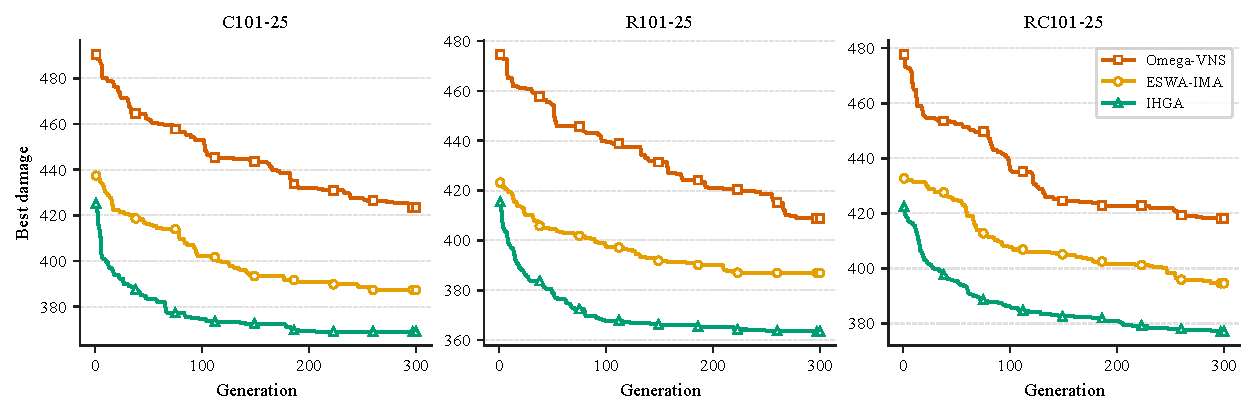
\includegraphics[width=0.98\textwidth]{figures/convergence_trace_eswa.pdf}
\caption{Convergence behaviour of Omega-VNS, ESWA-IMA, and IHGA on the representative C/R/RC instances under the unified dynamic damage objective.}
\label{fig:algorithm-convergence}
\end{figure}

Figure~\ref{fig:algorithm-convergence} reports the averaged best-so-far traces from the paper-lite convergence run. The curves should be interpreted as solution-quality evidence rather than as a computing-time comparison. On all three representative instance types, IHGA reaches a lower damage plateau than ESWA-IMA and Omega-VNS, which is consistent with the final statistics in Table~\ref{tab:algorithm-comparison}. The separation is especially useful for this study because it appears under clustered, random, and mixed customer layouts, suggesting that the proposed damage-critical and period-aware operators are not tuned only to one spatial pattern.

\begin{table}[H]
\centering
\caption{External algorithm robustness check on Homberger-derived 100-customer C/R/RC instances.}
\label{tab:algorithm-comparison-extended}
\scriptsize
\begin{tabular}{llrrr}
\toprule
Instance & Algorithm & Avg. damage & Best damage & Std. \\
\midrule
HC1-100 & VNS & 459.343 & 446.898 & 11.686 \\
HC1-100 & IMA & 424.700 & 420.107 & 7.040 \\
HC1-100 & IHGA & 411.557 & 411.398 & 0.263 \\
\midrule
HR1-100 & VNS & 445.411 & 436.060 & 8.326 \\
HR1-100 & IMA & 425.836 & 422.135 & 5.191 \\
HR1-100 & IHGA & 415.201 & 415.041 & 0.139 \\
\midrule
HRC1-100 & VNS & 436.001 & 431.155 & 4.583 \\
HRC1-100 & IMA & 418.580 & 415.246 & 4.946 \\
HRC1-100 & IHGA & 404.766 & 404.678 & 0.150 \\
\bottomrule
\end{tabular}
\end{table}

The external robustness check in Table~\ref{tab:algorithm-comparison-extended} follows the role of the larger comparison table in the original paper, but avoids treating time-window-only Solomon variants as independent spatial cases. IHGA obtains the lowest average damage on all three Homberger-derived C/R/RC instances. Across these runs, the average reduction is 2.96\% relative to IMA and 8.12\% relative to VNS. The minimum reduction is still positive on every external instance, indicating that the proposed operators remain useful outside the original three representative Solomon-type inputs.

\subsection{Algorithm ablation}
\label{subsec:operator-ablation}

The algorithm comparison shows that the proposed IHGA improves over the adapted IMA and VNS baselines, but this does not by itself identify which components are responsible for the gain. We therefore run an ablation study that keeps the same encoding and dynamic-damage evaluator, while selectively disabling the proposed repair components. The ``Base HGA'' variant removes the proposed damage-critical, period-aware, high-fleet, route-merge, route-rebuild, and polishing components. To keep the comparison paired, all variants use the same random seeds within each instance and repetition. Table~\ref{tab:operator-ablation} reports independent paired runs on the representative C/R/RC instances.

\begin{table}[H]
\centering
\caption{Ablation study of the proposed MP-IHGA search framework.}
\label{tab:operator-ablation}
\scriptsize
\begin{tabular}{llrrrr}
\toprule
Instance & Variant & Avg. damage & Best damage & Std. & Change vs MP-IHGA \\
\midrule
C101-25 & Base HGA & 378.369 & 376.376 & 2.156 & 2.49\% \\
C101-25 & w/o damage-critical & 373.905 & 370.095 & 4.357 & 1.28\% \\
C101-25 & w/o period relocation & 369.447 & 369.070 & 0.521 & 0.07\% \\
C101-25 & w/o route restructuring & 369.167 & 369.022 & 0.193 & 0.00\% \\
C101-25 & IHGA & 369.178 & 369.086 & 0.156 & 0.00\% \\
\midrule
r101-25 & Base HGA & 375.489 & 373.552 & 1.757 & 3.33\% \\
r101-25 & w/o damage-critical & 373.628 & 370.984 & 2.310 & 2.82\% \\
r101-25 & w/o period relocation & 364.029 & 363.468 & 0.498 & 0.18\% \\
r101-25 & w/o route restructuring & 364.125 & 363.441 & 0.816 & 0.21\% \\
r101-25 & IHGA & 363.376 & 363.052 & 0.487 & 0.00\% \\
\midrule
rc101-25 & Base HGA & 385.624 & 384.345 & 1.831 & 2.29\% \\
rc101-25 & w/o damage-critical & 380.461 & 380.308 & 0.214 & 0.92\% \\
rc101-25 & w/o period relocation & 377.745 & 375.801 & 2.696 & 0.20\% \\
rc101-25 & w/o route restructuring & 377.127 & 376.295 & 0.876 & 0.04\% \\
rc101-25 & IHGA & 376.992 & 376.388 & 0.744 & 0.00\% \\
\bottomrule

\end{tabular}
\end{table}

Table~\ref{tab:operator-ablation} is intended to answer a different question from Table~\ref{tab:algorithm-comparison}. Instead of asking whether MP-IHGA beats external baselines, it asks which proposed repair components are responsible for the improvement. The stripped Base HGA is clearly worse than the full method, showing that generic population search alone is insufficient. Damage-critical moves, period relocation, and route restructuring each contribute differently across clustered, random, and mixed layouts, which supports the interpretation that the final performance comes from combining multi-period and damage-aware search components rather than from a single parameter setting.

\subsection{Model comparison with CVRP and CCVRP}
\label{subsec:model-comparison}

To test whether dynamic damage must be modeled explicitly, we compare DDVRP-IHGA with two simplified multi-period baselines. The CVRP baseline minimizes total travel distance under the same capacity and period settings. The CCVRP baseline minimizes cumulative arrival time. After solving each baseline, the resulting routes are re-evaluated by the dynamic damage objective in Eq.~\eqref{eq:objective}. Table~\ref{tab:model-comparison} reports the resulting dynamic damage values and the improvement obtained by the proposed model.

\begin{table}[H]
\centering
\caption{Model comparison against distance-oriented CVRP and cumulative-arrival-time-oriented CCVRP.}
\label{tab:model-comparison}
\small
\begin{tabular}{lrrrrr}
\toprule
Instance & DDVRP-IHGA & CCVRP & CVRP & Improve vs CCVRP & Improve vs CVRP \\
\midrule
C101-25  & 369.037 & 462.896 & 494.251 & 20.28\% & 25.33\% \\
r101-25  & 362.770 & 429.711 & 494.436 & 15.58\% & 26.63\% \\
rc101-25 & 376.785 & 433.590 & 467.039 & 13.10\% & 19.33\% \\
\bottomrule
\end{tabular}
\end{table}

The results show that minimizing distance or cumulative arrival time is not sufficient for dynamic-damage reduction. CVRP is designed to shorten travel distance, and CCVRP is designed to reduce aggregate arrival time, but neither objective directly accounts for heterogeneous node vulnerability or road-damage-induced speed changes. The proposed damage-oriented model therefore produces lower dynamic damage on all three instance classes.

\begin{table}[H]
\centering
\caption{External model comparison on Homberger-derived 100-customer C/R/RC instances.}
\label{tab:model-comparison-extended}
\small
\begin{tabular}{lrrrrr}
\toprule
Instance & DDVRP-IHGA & CCVRP & CVRP & Improve vs CCVRP & Improve vs CVRP \\
\midrule
HC1-100 & 411.226 & 473.638 & 490.976 & 13.18\% & 16.24\% \\
HR1-100 & 414.910 & 468.294 & 475.631 & 11.40\% & 12.77\% \\
HRC1-100 & 404.695 & 443.222 & 478.549 & 8.69\% & 15.43\% \\
\bottomrule
\end{tabular}
\end{table}

The same conclusion holds in the external model-comparison table. DDVRP-IHGA produces lower dynamic damage than both simplified objectives on all reported external checks, with average reductions of 11.09\% relative to CCVRP and 14.81\% relative to CVRP. This supports the central modeling claim: shortest-distance and earliest-arrival objectives can be useful operational proxies, but they do not directly optimize the dynamic damage that the emergency decision maker ultimately seeks to reduce.

\subsection{Vehicle-number sensitivity analysis}
\label{subsec:vehicle-sensitivity}

Table~\ref{tab:vehicle-sensitivity} reports the sensitivity of total dynamic damage to the number of vehicles per period. The values are monotone decreasing on all three instances. From 6 to 50 vehicles per period, average damage decreases from 419.699 to 359.485 on C101-25, from 399.452 to 353.666 on r101-25, and from 410.112 to 367.130 on rc101-25.

\begin{table}[H]
\centering
\caption{Vehicle-number sensitivity results of IHGA.}
\label{tab:vehicle-sensitivity}
\scriptsize
\resizebox{\textwidth}{!}{%
\begin{tabular}{llrrrr}
\toprule
Instance & Vehicles/period & Avg. damage & Best damage & Std. & Runs \\
\midrule
C101-25 & 6  & 419.699 & 419.649 & 0.039 & 5 \\
C101-25 & 10 & 395.372 & 395.294 & 0.062 & 5 \\
C101-25 & 14 & 378.397 & 378.374 & 0.020 & 5 \\
C101-25 & 18 & 369.480 & 369.013 & 1.005 & 5 \\
C101-25 & 30 & 362.184 & 358.982 & 5.112 & 5 \\
C101-25 & 50 & 359.485 & 355.879 & 6.607 & 5 \\
\midrule
r101-25 & 6  & 399.452 & 399.186 & 0.236 & 5 \\
r101-25 & 10 & 382.500 & 381.976 & 0.446 & 5 \\
r101-25 & 14 & 370.895 & 370.370 & 0.344 & 5 \\
r101-25 & 18 & 362.500 & 361.877 & 0.443 & 5 \\
r101-25 & 30 & 355.484 & 354.106 & 1.776 & 5 \\
r101-25 & 50 & 353.666 & 352.486 & 1.189 & 5 \\
\midrule
rc101-25 & 6  & 410.112 & 409.648 & 0.423 & 5 \\
rc101-25 & 10 & 393.084 & 392.513 & 0.562 & 5 \\
rc101-25 & 14 & 382.778 & 382.594 & 0.148 & 5 \\
rc101-25 & 18 & 375.304 & 375.096 & 0.163 & 5 \\
rc101-25 & 30 & 369.279 & 367.982 & 0.965 & 5 \\
rc101-25 & 50 & 367.130 & 366.609 & 0.426 & 5 \\
\bottomrule
\end{tabular}%
}
\end{table}

\begin{figure}[H]
\centering
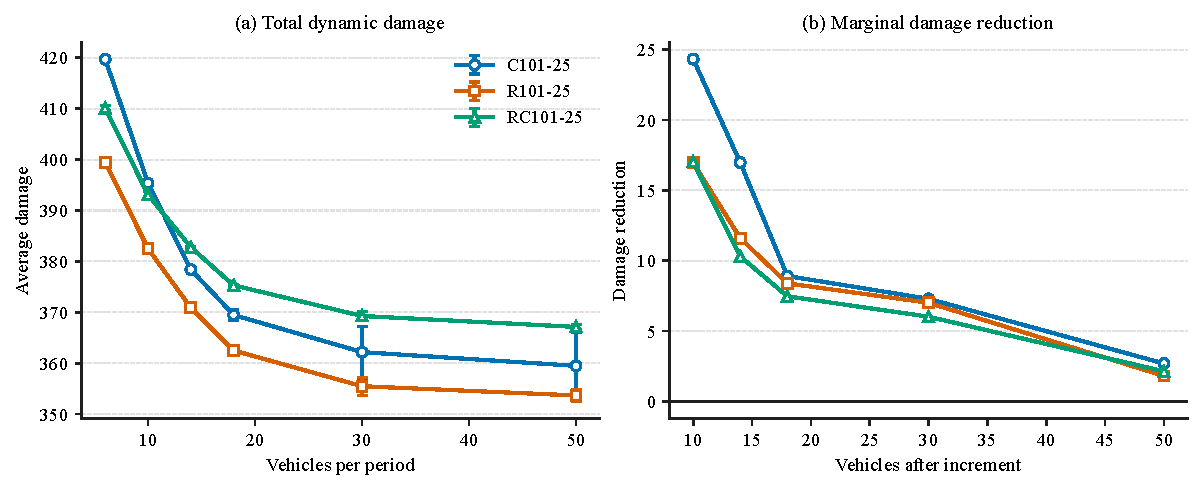
\includegraphics[width=0.95\textwidth]{figures/vehicle_sensitivity_eswa.pdf}
\caption{Vehicle-number sensitivity and marginal reductions. Panel (a) reports total dynamic damage, and panel (b) reports the marginal reduction between adjacent vehicle levels.}
\label{fig:vehicle-sensitivity}
\end{figure}

The marginal-reduction panel in Figure~\ref{fig:vehicle-sensitivity} further shows the diminishing-return pattern. The final interval from 30 to 50 vehicles reduces damage by only 0.745\% on C101-25, 0.511\% on r101-25, and 0.582\% on rc101-25. This supports a practical resource-allocation conclusion: increasing fleet size is most valuable when the fleet is scarce, while adding vehicles beyond a moderate level yields limited additional benefit.

\subsection{Multi-period dispatch and inventory sensitivity}
\label{subsec:period-inventory-sensitivity}

The period-sensitivity experiment is designed to isolate the importance of staged dispatch. We first add an optimistic single-period aggregate baseline, denoted by $P=1$, in which all 60 vehicles and the full relief inventory are available at the beginning of the horizon. This is not intended to represent a realistic post-earthquake operation. It is a lower-bound reference for the plan that would be obtained if disrupted roads and upstream supply constraints did not delay resource availability. We then vary the number of staged dispatch periods while keeping the total fleet fixed at 60 vehicles and keeping total supply approximately equal to total demand. Therefore, increasing the number of staged periods does not add resources; instead, it splits the same vehicles and the same total supply into more dispatch waves, reducing both the vehicles per period and the inventory available in each early period.

Table~\ref{tab:period-sensitivity} reports both the optimistic aggregate baseline and the staged-dispatch settings. The percentage column measures the extra dynamic damage relative to the $P=1$ aggregate baseline.

\begin{table}[H]
\centering
\caption{Period sensitivity with an optimistic aggregate baseline and fixed-total staged resources.}
\label{tab:period-sensitivity}
\scriptsize
\resizebox{\textwidth}{!}{%
\begin{tabular}{lllrrrrrrr}
\toprule
Instance & Periods & Scenario & Vehicles/period & Total vehicles & $Q_p$ & Total supply & Total demand & Avg. damage & Increase vs $P=1$ \\
\midrule
C101-25 & 1 & Aggregate & 60 & 60 & 1810 & 1810 & 1810 & 343.953 & 0.00\% \\
C101-25 & 2 & Staged & 30 & 60 & 905 & 1810 & 1810 & 352.485 & 2.48\% \\
C101-25 & 3 & Staged & 20 & 60 & 604 & 1812 & 1810 & 364.909 & 6.09\% \\
C101-25 & 4 & Staged & 15 & 60 & 453 & 1812 & 1810 & 376.536 & 9.47\% \\
C101-25 & 5 & Staged & 12 & 60 & 362 & 1810 & 1810 & 385.990 & 12.22\% \\
\midrule
r101-25 & 1 & Aggregate & 60 & 60 & 1458 & 1458 & 1458 & 341.987 & 0.00\% \\
r101-25 & 2 & Staged & 30 & 60 & 729 & 1458 & 1458 & 350.881 & 2.60\% \\
r101-25 & 3 & Staged & 20 & 60 & 486 & 1458 & 1458 & 360.558 & 5.43\% \\
r101-25 & 4 & Staged & 15 & 60 & 365 & 1460 & 1458 & 369.321 & 7.99\% \\
r101-25 & 5 & Staged & 12 & 60 & 292 & 1460 & 1458 & 377.408 & 10.36\% \\
\midrule
rc101-25 & 1 & Aggregate & 60 & 60 & 1724 & 1724 & 1724 & 362.440 & 0.00\% \\
rc101-25 & 2 & Staged & 30 & 60 & 862 & 1724 & 1724 & 366.159 & 1.03\% \\
rc101-25 & 3 & Staged & 20 & 60 & 575 & 1725 & 1724 & 373.404 & 3.03\% \\
rc101-25 & 4 & Staged & 15 & 60 & 431 & 1724 & 1724 & 381.889 & 5.37\% \\
rc101-25 & 5 & Staged & 12 & 60 & 345 & 1725 & 1724 & 390.287 & 7.68\% \\
\bottomrule
\end{tabular}%
}
\end{table}

\begin{figure}[H]
\centering
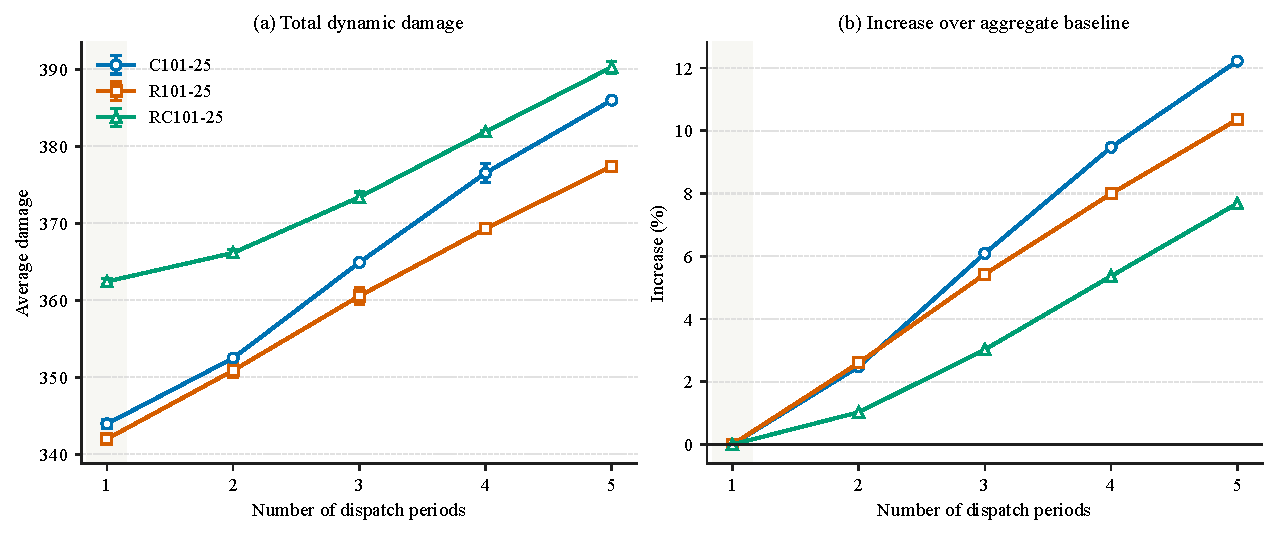
\includegraphics[width=0.95\textwidth]{figures/period_sensitivity_eswa.pdf}
\caption{Period sensitivity under an optimistic aggregate baseline ($P=1$) and staged fixed-total resources ($P\ge2$). The shaded first period marks the aggregate lower-bound reference.}
\label{fig:period-sensitivity}
\end{figure}

As expected, the aggregate baseline has the lowest damage because it assumes that all resources can be dispatched immediately. Relative to this optimistic lower bound, the default three-period setting increases average damage by 6.09\% on C101-25, 5.43\% on r101-25, and 3.03\% on rc101-25. With five staged periods, the increases reach 12.22\%, 10.36\%, and 7.68\%, respectively. Among the realistic staged settings, moving from two to five periods raises damage by 9.51\% on C101-25, 7.56\% on r101-25, and 6.59\% on rc101-25. This does not imply that more periods are intrinsically harmful. Rather, under the fixed-total-resource design, more periods mean fewer vehicles and less supply in each early period, which weakens early service capability. The result highlights why multi-period modeling matters: if a post-earthquake response is forced to receive vehicles and materials in waves, a single-period aggregate model hides the loss caused by delayed resource availability.

\begin{figure}[H]
\centering
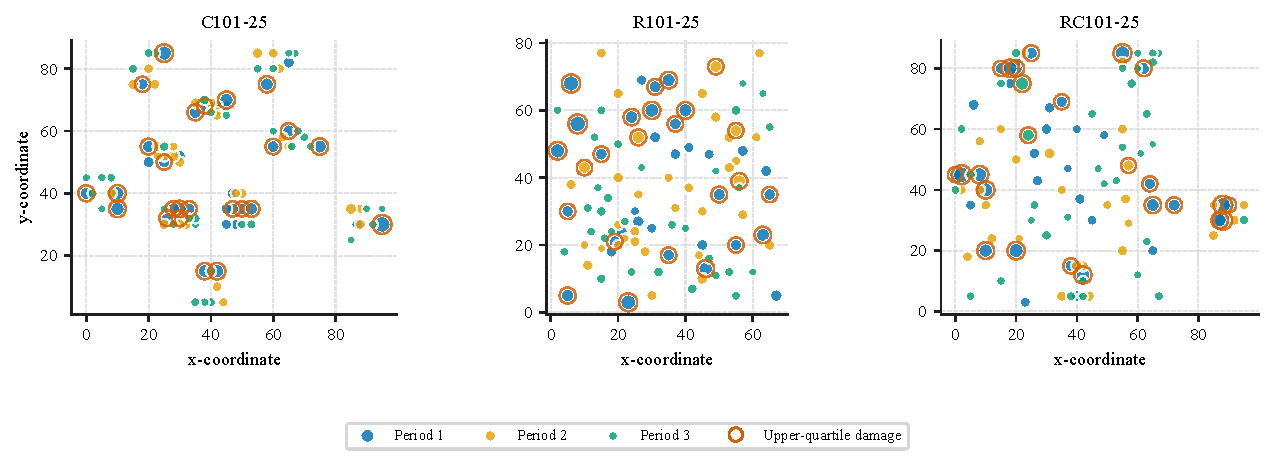
\includegraphics[width=0.95\textwidth]{figures/service_period_map_eswa.pdf}
\caption{Service-period assignment in representative three-period IHGA route-plan exports. Colors indicate the period in which each demand node is first served; outer rings mark nodes in the upper quartile of realized dynamic damage.}
\label{fig:service-period-map}
\end{figure}

Figure~\ref{fig:service-period-map} gives a solution-level view of the same modeling issue. The map is not a conceptual sketch; it is generated from the exported IHGA route plans. Nodes with high realized damage are not confined to one geometric cluster, and some must still be served in later periods because each period has limited vehicles and inventory. This is precisely the case in which a single-period aggregate plan becomes optimistic: it can hide the timing constraint by assuming that all vehicles and materials are available immediately.

The inventory-sensitivity experiment fixes $P=3$ and the total fleet at 60 vehicles, then varies the per-period inventory quantity $Q_p$. This experiment separates the effect of total supply sufficiency from the effect of period-level availability. Table~\ref{tab:inventory-sensitivity} reports the feasible region where cumulative supply is at least total demand. The under-supply setting with $Q_p$ below the feasible threshold is excluded from the linear-scale table because it activates the large penalty term in Eq.~\eqref{eq:objective}.

\begin{table}[H]
\centering
\caption{Inventory sensitivity in the feasible supply region.}
\label{tab:inventory-sensitivity}
\small
\begin{tabular}{lrrrrr}
\toprule
Instance & $Q_p$ & Total supply & Total demand & Supply factor & Avg. damage \\
\midrule
C101-25 & 604 & 1812 & 1810 & 1.000 & 365.176 \\
C101-25 & 725 & 2175 & 1810 & 1.200 & 364.935 \\
C101-25 & 906 & 2718 & 1810 & 1.500 & 364.828 \\
\midrule
r101-25 & 486 & 1458 & 1458 & 1.000 & 360.421 \\
r101-25 & 584 & 1752 & 1458 & 1.202 & 359.751 \\
r101-25 & 729 & 2187 & 1458 & 1.500 & 359.198 \\
\midrule
rc101-25 & 575 & 1725 & 1724 & 1.000 & 373.368 \\
rc101-25 & 690 & 2070 & 1724 & 1.200 & 372.743 \\
rc101-25 & 863 & 2589 & 1724 & 1.501 & 372.632 \\
\bottomrule
\end{tabular}
\end{table}

After the feasibility threshold is reached, additional inventory produces limited marginal improvement. For example, increasing the supply factor from 1.0 to approximately 1.2 reduces average damage by 0.242 on C101-25, 0.671 on r101-25, and 0.625 on rc101-25. Increasing from approximately 1.2 to 1.5 produces even smaller reductions on C101-25 and rc101-25. When total supply is only about 0.8 times total demand, the shortage-penalty term dominates the objective and raises the average objective to the order of $10^6$. These shortage cases are therefore treated as infeasible stress checks rather than plotted together with the feasible marginal-effect results. Together with the period-sensitivity results, this indicates that multi-period planning is most valuable for identifying the early-resource bottleneck: once every period has enough feasible supply, simply increasing inventory is much less effective than improving early dispatch capacity.

\subsection{Priority analysis}
\label{subsec:priority-analysis}

The original DCCVRPMRS benchmark also compares the proposed model with heuristic delivery strategies that strictly prioritize either the highest initial damage or the highest deterioration rate. To provide the corresponding evidence, we construct two priority-only baselines under the same vehicle-capacity and period-inventory constraints. In each baseline, nodes are sorted by the selected priority indicator and assigned to the earliest feasible route, and the resulting routes are then evaluated by the same dynamic-damage objective. Table~\ref{tab:priority-strategy} reports the comparison on the same Homberger-derived external set used in Tables~\ref{tab:algorithm-comparison-extended} and \ref{tab:model-comparison-extended}.

\begin{table}[H]
\centering
\caption{Comparison with priority-only heuristic delivery strategies.}
\label{tab:priority-strategy}
\scriptsize
\resizebox{\textwidth}{!}{%
\begin{tabular}{lrrrrr}
\toprule
Instance & DDVRP-IHGA & Initial-damage priority & Deterioration priority & Improve vs initial & Improve vs deterioration \\
\midrule
HC1-100 & 411.557 & 473.858 & 488.270 & 13.15\% & 15.71\% \\
HR1-100 & 415.201 & 465.707 & 487.061 & 10.85\% & 14.75\% \\
HRC1-100 & 404.766 & 464.157 & 485.060 & 12.80\% & 16.55\% \\
\bottomrule
\end{tabular}%
}
\end{table}

IHGA outperforms both priority-only strategies on all reported external entries, with average reductions of 12.26\% relative to the initial-damage priority rule and 15.67\% relative to the deterioration-rate priority rule. This result supports the same qualitative conclusion as the original priority-strategy experiment: considering one urgency factor alone is not enough. The route plan must balance initial damage, deterioration, travel delay, road condition, vehicle capacity, and period-level inventory timing.

The second priority analysis divides nodes into low, medium, and high groups according to the integrated urgency score used by IHGA. Table~\ref{tab:priority-analysis} reports average arrival time, average service rank, and average node damage for the three groups. A lower service rank indicates earlier service.

\begin{table}[H]
\centering
\caption{Urgency-based priority analysis.}
\label{tab:priority-analysis}
\scriptsize
\resizebox{\textwidth}{!}{%
\begin{tabular}{lrrrrrrrrr}
\toprule
Instance & Arrival high & Arrival medium & Arrival low & Rank high & Rank medium & Rank low & Damage high & Damage medium & Damage low \\
\midrule
C101-25  & 78.217 & 575.125 & 997.021 & 19.200 & 52.939 & 80.309 & 5.844 & 3.200 & 1.961 \\
r101-25  & 97.577 & 550.313 & 800.502 & 22.288 & 56.891 & 73.176 & 5.681 & 3.187 & 1.961 \\
rc101-25 & 68.253 & 559.239 & 900.300 & 19.559 & 55.679 & 77.200 & 6.047 & 3.200 & 1.961 \\
\bottomrule
\end{tabular}%
}
\end{table}

High-urgency nodes are served much earlier than low-urgency nodes on all three instances. Their average arrival time is 92.16\% earlier than low-urgency nodes on C101-25, 87.81\% earlier on r101-25, and 92.42\% earlier on rc101-25. The high-urgency group still has larger average node damage because these nodes have larger intrinsic vulnerability. Therefore, the result should be interpreted as evidence that IHGA prioritizes vulnerable nodes rather than as a failure to reduce their loss completely.

\section{Conclusion}
\label{sec:conclusion}

This paper studies a multi-period vehicle routing problem with dynamic node-road damage for emergency material delivery. The model captures three key features of post-disaster routing: node losses depend on arrival time, road damage affects travel speed and downstream service times, and vehicles and inventories are released through dispatch periods rather than being fully available at the beginning of the horizon. An improved hybrid genetic algorithm is developed to solve the problem. In addition to standard genetic and local-search components, IHGA uses urgency-aware construction, route-similarity crossover, damage-critical relocation and exchange, period-aware relocation, high-fleet parallel relocation, route merging, route rebuilding, and warm-start transfer.

Computational experiments on C101-25, r101-25, and rc101-25 demonstrate the effectiveness and interpretability of the proposed method. IHGA consistently obtains lower average dynamic damage than Omega-VNS and ESWA-IMA. External checks on Homberger-derived 100-customer C/R/RC instances further show that this advantage is not limited to the three representative instances. The ablation study shows that the improvement is not only due to generic genetic search: the stripped Base HGA is clearly worse than the full method, and the proposed repair components contribute to damage reduction across representative layouts. The damage-oriented model also outperforms distance-oriented CVRP and cumulative-arrival-time-oriented CCVRP baselines, confirming that distance or arrival time alone is not a sufficient proxy for emergency loss. The multi-period sensitivity results show that total resource quantity and resource timing are not interchangeable. The aggregate single-period baseline gives an optimistic lower bound, while staged dispatch produces additional dynamic damage when the same total fleet and total supply become available through later waves. Inventory experiments show a complementary threshold effect: severe under-supply creates infeasible penalty-dominated solutions, whereas additional inventory beyond the feasible threshold yields only limited marginal improvement. Priority experiments further show that one-factor priority rules are inferior to the integrated dynamic-damage objective, while the urgency-group analysis verifies that high-urgency nodes are served substantially earlier than low-urgency nodes.

Future work can extend the current deterministic setting to stochastic demand, uncertain road recovery, and rolling-horizon dispatch with real-time information updates. Larger benchmark instances and richer disaster-network data can also be used to further test scalability and operational realism.

\appendix
\section{Implementation notes}
\label{app:implementation}

The current MATLAB implementation evaluates each route by recursively updating arrival times and node damage. Route indices are fixed by period, so empty routes are retained rather than removed. This design prevents accidental period-index changes during local search. The vehicle-number sensitivity runner uses the best solution from a smaller fleet as a warm start for the next larger fleet.

\bibliographystyle{elsarticle-harv}
\bibliography{mybib}

\end{document}




